\documentclass[11pt,a4paper]{article}

% -------------------- PACKAGES --------------------
\usepackage[utf8]{inputenc}
\usepackage[T1]{fontenc}
\usepackage[english]{babel}
\usepackage{amsmath,amssymb,mathtools}
\usepackage{graphicx}
\usepackage{float}
\usepackage{geometry}
\usepackage{setspace}
\usepackage[table,xcdraw]{xcolor}
\usepackage{booktabs}
\usepackage{array}
\usepackage{enumitem}
\usepackage{caption}
\usepackage{hyperref}
\usepackage{tikz}
\usepackage{fancyhdr}
\usepackage{tcolorbox}
\usepackage{listings}
\tcbuselibrary{skins,breakable}
\usetikzlibrary{shapes.geometric,arrows.meta,positioning,calc}

% -------------------- GENERAL SETUP --------------------
\geometry{top=1.8cm,bottom=1.8cm,left=1.8cm,right=1.8cm,headheight=1.2cm}
\setstretch{1.04}
\setlength{\parindent}{0pt}
\setlength{\parskip}{0.30em}
\captionsetup{font=small,skip=3pt}


\hypersetup{
  hidelinks,
  colorlinks=true,
  urlcolor=blue,
  citecolor=blue,
  linkcolor=black,
  breaklinks=true
}

% -------------------- COLORS --------------------
\definecolor{softGray}{RGB}{248,249,250}
\definecolor{softBlue}{RGB}{239,246,255}
\definecolor{softGreen}{RGB}{239,250,244}
\definecolor{lineGray}{RGB}{190,198,208}
\definecolor{deepBlue}{RGB}{30,64,175}
\definecolor{deepGreen}{RGB}{21,128,61}
\definecolor{deepAmber}{RGB}{180,83,9}
\definecolor{codeBg}{RGB}{246,248,250}
\definecolor{codeFrame}{RGB}{220,225,232}

% -------------------- LISTINGS SETUP --------------------
\lstdefinestyle{codeStyle}{
  backgroundcolor=\color{codeBg},
  basicstyle=\ttfamily\scriptsize,
  breakatwhitespace=false,
  breaklines=true,
  captionpos=b,
  keepspaces=true,
  numbers=left,
  numbersep=5pt,
  numberstyle=\tiny\color{gray},
  showspaces=false,
  showstringspaces=false,
  frame=single,
  rulecolor=\color{codeFrame},
  keywordstyle=\color{deepBlue}\bfseries,
  commentstyle=\color{deepGreen}\itshape,
  stringstyle=\color{deepAmber}
}

% -------------------- HEADER / FOOTER --------------------
\pagestyle{fancy}
\fancyhf{}
\fancyhead[L]{\small\textit{Distributed Systems --- Workshop 3: Naming}}
\fancyhead[R]{\small\textit{Yachay Tech University}}
\fancyfoot[C]{\thepage}
\renewcommand{\headrulewidth}{0.4pt}

% -------------------- BOXES --------------------
\newtcolorbox{conceptbox}[1][]{enhanced,
  colback=softBlue,colframe=deepBlue,
  fonttitle=\bfseries\small,title={#1},
  left=6pt,right=6pt,top=5pt,bottom=5pt}

\newtcolorbox{solutionbox}[1][]{enhanced,
  colback=softGreen,colframe=deepGreen,
  fonttitle=\bfseries\small,title={#1},
  left=6pt,right=6pt,top=5pt,bottom=5pt}

\newcommand{\safeincludegraphics}[2]{%
  \IfFileExists{#2}{\includegraphics[#1]{#2}}{%
    \fbox{\begin{minipage}[c][1.5cm][c]{0.45\textwidth}
      \centering\small Missing image: \texttt{\detokenize{#2}}
    \end{minipage}}}}

% ================================================================
\begin{document}
% ================================================================

% -------------------- TITLE / COVER HEADER --------------------
\begin{minipage}{0.48\textwidth}
  \flushleft
  \safeincludegraphics{width=0.36\textwidth}{Imagenes/logo1.png}
\end{minipage}
\hfill
\begin{minipage}{0.48\textwidth}
  \flushright
  \safeincludegraphics{width=0.40\textwidth}{Imagenes/logo2.png}
\end{minipage}

\vspace{0.3cm}

\begin{center}
  {\LARGE\bfseries Workshop 3: Naming}\\[3pt]
  {\large\bfseries Distributed Systems --- Practical Report}\\[8pt]
  \textbf{Authors:} Dario Pomasqui \quad \& \quad Adriana Sofia Espinoza Chicaiza\\
  \textit{School of Mathematical and Computational Sciences, Yachay Tech University}\\
  \textbf{Professor:} Francisco Hidrobo, Ph.D. \quad $\vert$ \quad \textbf{Date:} September 03, 2026
\end{center}
\vspace{-0.2cm}
\hrule
\vspace{0.4cm}

% ================================================================
\section{Theoretical Framework}
% ================================================================

In distributed systems, accessing resources and communication endpoints fundamentally requires resolving an identification token to an operational access point \cite{tanenbaum, coulouris}. Literature distinguishes three core concepts:
\begin{itemize}[leftmargin=*,itemsep=1pt]
  \item \textbf{Name:} A human-friendly or symbolic label for an entity (e.g., DNS hostname \texttt{student-a.lan}).
  \item \textbf{Identifier:} A location-independent, unique bit string (e.g., UUIDv5) that refers to at most one entity, is never reused, and never changes even when the entity relocates.
  \item \textbf{Address:} A location-dependent network contact point (e.g., IPv4 tuple \texttt{(192.168.1.14, 5000)} or MAC address) used by routing protocols to deliver packets.
\end{itemize}

\begin{conceptbox}[Naming Paradigms Evaluated in Workshop 3]
\begin{itemize}[leftmargin=*,itemsep=1pt]
  \item \textbf{Flat Naming:} Identifiers have no internal structure or topological clues. Resolution relies on: (1)~\textit{Broadcasting} (LAN-only flooding), (2)~\textit{Forwarding Pointers} (movement chains with shortcut optimizations), and (3)~\textit{Distributed Hash Tables (DHTs)} like Chord ($O(\log N)$ routing).
  \item \textbf{Structured / Hierarchical Naming:} Names are organized into hierarchical domain trees (e.g., Hierarchical Location Services [HLS]) or directed naming graphs (e.g., POSIX file systems with hard and soft links).
\end{itemize}
\end{conceptbox}

% ================================================================
\section{Exercise 1 --- Identifiers vs. Addresses}
% ================================================================

\textbf{Objective:} Decouple entity identity from network location and verify that an entity identifier remains invariant under address reassignment.

\textbf{Implementation and Evidence:} In \texttt{identifiers.py}, a deterministic UUIDv5 is generated from \texttt{"student-a"} in the DNS namespace, while the IP address is discovered dynamically. The entity records its address at port 5000 and is subsequently reassigned to port 6000:

\begin{figure}[H]
  \centering
  \safeincludegraphics{width=0.78\textwidth}{Imagenes/ejercicio1_terminal.png}
  \caption{Terminal output of \texttt{identifiers.py}: the UUID remains constant while the port address is modified.}
  \label{fig:ej1}
\end{figure}

\begin{solutionbox}[Why UUID Alone is Insufficient for Communication]
When Student A provides only the UUID (\texttt{fc1ce712-f56d-5831-be86-2b82ea445f5a}), Student B cannot initiate direct communication because:
\begin{enumerate}[leftmargin=*,itemsep=1pt]
  \item \textbf{Zero Routing Semantics:} Transport and network layer protocols require topological endpoints (IP address, transport port, MAC address). A UUID contains no subnet or gateway routing data.
  \item \textbf{Separation of Concerns:} An identifier specifies \textit{which} entity is targeted, while an address specifies \textit{where} it is currently hosted.
  \item \textbf{Mobility and Rebinding:} When the port changes from 5000 to 6000, communication without an active lookup service would fail. An explicit resolution mechanism ($\text{UUID} \mapsto (\text{IP}, \text{Port})$) is mandatory.
\end{enumerate}
\end{solutionbox}

% ================================================================
\section{Exercise 2 --- Locating an Entity by Broadcast}
% ================================================================

\textbf{Objective:} Study flat name resolution through broadcast at the Link Layer (ARP) and Application Layer (UDP sockets).

\subsection{Link-Layer Resolution (ARP / Neighbor Cache)}
Inspecting the operating system's ARP table (\texttt{arp -a}) reveals the dynamic binding between logical IPv4 addresses and physical Layer-2 MAC addresses. Pinging the local gateway triggers ARP requests and populates the cache:

\begin{figure}[H]
  \centering
  \safeincludegraphics{width=0.78\textwidth}{Imagenes/ejercicio2_arp.png}
  \caption{Link-layer evidence: IPv4 configuration, ARP neighbor table, and ICMP ping verification.}
  \label{fig:ej2_arp}
\end{figure}

\subsection{Application-Level UDP Broadcast}
At the application layer, \texttt{entity.py} (Student A) listens on UDP port 50000, while \texttt{finder.py} (Student B) broadcasts to \texttt{255.255.255.255:50000}.
\begin{itemize}[leftmargin=*,itemsep=1pt]
  \item \textbf{Successful Discovery:} Querying \texttt{"studentA-Name"} returns \texttt{"studentA-Name:192.168.1.14"}.
  \item \textbf{Unsuccessful Discovery:} Querying non-existent \texttt{"studentB-Name"} causes a 3-second socket timeout resulting in \texttt{"Entity not found"}.
\end{itemize}

\begin{figure}[H]
  \centering
  \safeincludegraphics{width=0.78\textwidth}{Imagenes/ejercicio2_broadcast.png}
  \caption{Real terminal capture of UDP broadcast resolution: Student A listener, Student B success, and Student B timeout.}
  \label{fig:ej2_broadcast}
\end{figure}

\textbf{Scalability Limitations:} Broadcasting does not scale in distributed systems because: (1) \textit{CPU Interrupt Storms:} Every node on the LAN must interrupt its processor to inspect every broadcast frame ($O(N)$ network overhead); (2) \textit{Router Boundaries:} Routers deliberately drop link-local broadcast packets, confining resolution strictly to a single local subnet.

% ================================================================
\section{Exercise 3 --- Forwarding Pointers}
% ================================================================

\textbf{Objective:} Trace forwarding pointer chains, implement the shortcut optimization, and simulate intermediate link failure.

\textbf{Implementation and Evidence:} In \texttt{forwarding.py}, an entity moves through locations $A \to B \to C \to D \to \text{Address}$.
\begin{itemize}[leftmargin=*,itemsep=1pt]
  \item \textbf{Unoptimized Chain:} Traversing all intermediate pointers requires \textbf{4 hops}.
  \item \textbf{Shortcut Optimization:} Updating $A$'s pointer directly to the final address (\texttt{locations["A"] = address}) compresses resolution to \textbf{1 hop} (a $75\%$ reduction in lookup latency).
  \item \textbf{Failure Simulation:} Deleting intermediate node $C$ (\texttt{del locations["C"]}) severs the original pointer chain ($A \to B \to C \to \text{Halt}$), preventing callers relying on the legacy path from reaching the target entity.
\end{itemize}

\begin{figure}[H]
  \centering
  \safeincludegraphics{width=0.78\textwidth}{Imagenes/ejercicio3_forwarding.png}
  \caption{Terminal output of \texttt{forwarding.py}: 4-hop resolution, 1-hop shortcut, and chain failure simulation.}
  \label{fig:ej3}
\end{figure}

\begin{table}[H]
\centering
\caption{Forwarding pointer resolution metrics}
\label{tab:forwarding_metrics}
\small
\begin{tabular}{lccc}
\toprule
\textbf{Test Configuration} & \textbf{Traversal Path} & \textbf{Hops} & \textbf{Resolution Status} \\
\midrule
Unoptimized Chain & $A \to B \to C \to D \to 192.168.1.50:5000$ & 4 & Successful \\
Shortcut Optimization & $A \to 192.168.1.50:5000$ & 1 & Successful ($75\%$ latency reduction) \\
Intermediate Failure ($\text{del } C$) & $A \to B \to C \to \text{HALT}$ & 2 & \textbf{Broken Chain (Failure)} \\
\bottomrule
\end{tabular}
\end{table}

\textbf{Discussion:} While forwarding pointers provide $O(1)$ update cost during migration, long chains accumulate network round-trip delays ($O(k)$ RTT) and suffer high vulnerability: a single crashed intermediary breaks client access permanently unless shortcuts and garbage collection are maintained.

% ================================================================
\section{Exercise 4 --- Implementing a Simplified Chord Ring}
% ================================================================

\textbf{Objective:} Implement a Distributed Hash Table (DHT) based on Chord consistent hashing with $m=5$ ($2^5=32$ positions), compute finger tables, and route lookups in $O(\log N)$ hops \cite{chord}.

\subsection{Mathematical Model and Ring Setup}
\begin{itemize}[leftmargin=*,itemsep=1pt]
  \item \textbf{Identifier Circle:} Positions $0 \dots 31 \pmod{32}$. Active nodes: $\mathcal{N} = \{1, 4, 9, 11, 14, 18, 20, 21, 28\}$.
  \item \textbf{Successor Rule:} Key $k$ is stored at the smallest node $\ge k \pmod{32}$: $\text{succ}(k) = \min \{ n \in \mathcal{N} \mid n \ge k \}$.
  \item \textbf{Finger Table:} For node $p$, entry $i$ ($1 \le i \le 5$) points to $FT_p[i] = \text{succ}((p + 2^{i-1}) \bmod 32)$.
\end{itemize}

\subsection{Successor Mapping and Finger Tables}

\begin{table}[H]
\centering
\begin{minipage}{0.45\textwidth}
\caption{Part A: Key-to-Node Mapping}
\label{tab:chord_partA}
\centering\footnotesize
\begin{tabular}{ccl}
\toprule
\textbf{Key} & \textbf{Node} & \textbf{Justification} \\
\midrule
3  & 4  & Smallest node $\ge 3$ \\
8  & 9  & Smallest node $\ge 8$ \\
12 & 14 & Nodes $9,11 < 12 \implies 14$ \\
19 & 20 & Smallest node $\ge 19$ \\
26 & 28 & Smallest node $\ge 26$ \\
30 & 1  & Wraps around modulo 32 \\
\bottomrule
\end{tabular}
\end{minipage}
\hfill
\begin{minipage}{0.52\textwidth}
\caption{Part B: Finger Tables ($FT_p$)}
\label{tab:chord_fingers}
\centering\footnotesize
\begin{tabular}{cccccc}
\toprule
\textbf{Node} & \textbf{+1} & \textbf{+2} & \textbf{+4} & \textbf{+8} & \textbf{+16} \\
\midrule
1  & 4  & 4  & 9  & 9  & 18 \\
4  & 9  & 9  & 9  & 14 & 20 \\
9  & 11 & 11 & 14 & 18 & 28 \\
11 & 14 & 14 & 18 & 20 & 28 \\
14 & 18 & 18 & 18 & 28 & 1  \\
18 & 20 & 20 & 28 & 28 & 4  \\
20 & 21 & 28 & 28 & 28 & 4  \\
21 & 28 & 28 & 28 & 1  & 9  \\
28 & 1  & 1  & 1  & 4  & 14 \\
\bottomrule
\end{tabular}
\end{minipage}
\end{table}

\subsection{Routing Execution and Ring Topology}
\begin{itemize}[leftmargin=*,itemsep=1pt]
  \item \textbf{Lookup Key 26 from Node 1:} $1 \xrightarrow{FT_1[5]} 18 \xrightarrow{FT_{18}[2]} 20 \xrightarrow{FT_{20}[1]} 21 \xrightarrow{\text{succ}} 28$ (\textbf{4 hops}).
  \item \textbf{Lookup Key 12 from Node 28:} $28 \xrightarrow{FT_{28}[4]} 4 \xrightarrow{FT_4[3]} 9 \xrightarrow{FT_9[1]} 11 \xrightarrow{\text{succ}} 14$ (\textbf{4 hops}).
\end{itemize}

\begin{figure}[H]
  \centering
  \begin{minipage}{0.48\textwidth}
    \centering
    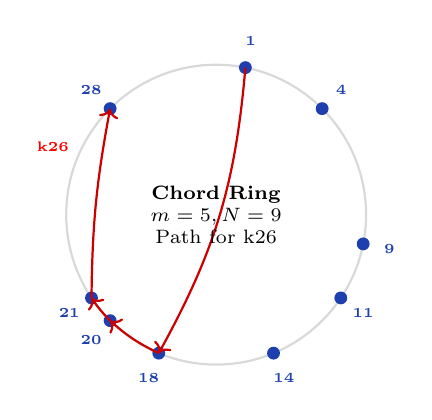
\begin{tikzpicture}[scale=0.68]
      \draw[thick, gray!30] (0,0) circle (2.8cm);
      \foreach \i in {0,...,31} {
        \pgfmathsetmacro{\angle}{90 - \i * (360 / 32)}
        \coordinate (P\i) at (\angle:2.8cm);
        \coordinate (L\i) at (\angle:3.3cm);
      }
      \foreach \n in {1, 4, 9, 11, 14, 18, 20, 21, 28} {
        \fill[deepBlue] (P\n) circle (0.12cm);
        \node[font=\tiny\bfseries, deepBlue] at (L\n) {\n};
      }
      \node[red, font=\tiny\bfseries] at (L26) {k26};
      \draw[->, thick, red!80!black] (P1) to[bend left=12] (P18);
      \draw[->, thick, red!80!black] (P18) to[bend left=8] (P20);
      \draw[->, thick, red!80!black] (P20) to[bend left=5] (P21);
      \draw[->, thick, red!80!black] (P21) to[bend left=5] (P28);
      \node at (0,0) [align=center, font=\scriptsize] {\textbf{Chord Ring}\\$m=5, N=9$\\Path for k26};
    \end{tikzpicture}
    \caption{Chord logical ring topology.}
    \label{fig:chord_diagram}
  \end{minipage}
  \hfill
  \begin{minipage}{0.50\textwidth}
    \centering
    \safeincludegraphics{width=\textwidth}{Imagenes/ejercicio4_chord.png}
    \caption{Terminal execution of \texttt{chord.py}.}
    \label{fig:ej4_terminal}
  \end{minipage}
\end{figure}

% ================================================================
\section{Exercise 5 --- Hierarchical Location Service (HLS)}
% ================================================================

\textbf{Objective:} Model a worldwide network hierarchy using administrative domains, downward pointers, and locality-aware search.

\subsection{Architecture and Lookup Principles}
The namespace is partitioned into a tree: $\text{ROOT} \to \{\text{AMERICA}, \text{EUROPE}\}$, $\text{AMERICA} \to \{\text{ECUADOR}, \text{USA}\}$, $\text{ECUADOR} \to \{\text{IBARRA}, \text{QUITO}\}$. Leaves store entity addresses; intermediate directory nodes maintain \textbf{downward pointers} to child subtrees containing entities.

\begin{figure}[H]
  \centering
  \begin{minipage}{0.46\textwidth}
    \centering
    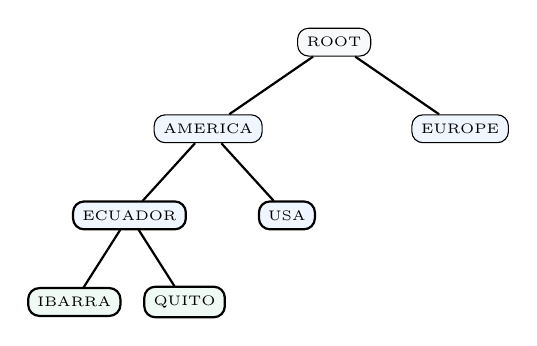
\begin{tikzpicture}[
      level 1/.style={sibling distance=3.2cm, level distance=1.1cm},
      level 2/.style={sibling distance=2.0cm, level distance=1.1cm},
      level 3/.style={sibling distance=1.4cm, level distance=1.1cm},
      every node/.style={draw, rounded corners, fill=softBlue, font=\tiny, align=center},
      edge from parent/.style={draw, thick, -}
    ]
      \node[fill=softGray] {ROOT}
        child { node {AMERICA}
          child { node {ECUADOR}
            child { node[fill=softGreen] {IBARRA} }
            child { node[fill=softGreen] {QUITO} }
          }
          child { node {USA} }
        }
        child { node {EUROPE} };
    \end{tikzpicture}
    \caption{HLS domain tree hierarchy.}
    \label{fig:hls_tree}
  \end{minipage}
  \hfill
  \begin{minipage}{0.52\textwidth}
    \centering
    \safeincludegraphics{width=\textwidth}{Imagenes/ejercicio5_hls.png}
    \caption{Terminal execution of \texttt{hls.py}.}
    \label{fig:ej5_terminal}
  \end{minipage}
\end{figure}

\subsection{Evaluation of Locality and Entity Relocation}
\begin{enumerate}[leftmargin=*,itemsep=1pt]
  \item \textbf{Exploitation of Locality:} Resolving \texttt{server02} from \texttt{IBARRA} moves upward only to \texttt{ECUADOR} (the Lowest Common Ancestor, LCA), which contains a downward pointer directly to \texttt{QUITO}. It \textbf{never contacts} \texttt{AMERICA} or \texttt{ROOT}, completely shielding global nodes from regional query traffic.
  \item \textbf{Search Boundary for Absent Entities:} Querying non-existent \texttt{server99} ascends all the way to \texttt{ROOT} before terminating with \texttt{"Entity not found"}.
  \item \textbf{Localized Migration Cost:} Relocating \texttt{server01} from \texttt{IBARRA} to \texttt{QUITO} (address \texttt{10.0.2.25}) only modifies records within \texttt{ECUADOR} and the leaves. Pointers at \texttt{AMERICA} and \texttt{ROOT} remain untouched, proving minimal update signaling overhead.
\end{enumerate}

% ================================================================
\section{Exercise 6 --- Name Spaces, Inodes, Hard and Soft Links}
% ================================================================

\textbf{Objective:} Analyze graph-theoretic namespace resolution by comparing hard links (direct inode references) with soft links (indirect symbolic path pointers) under file rename and deletion.

\begin{figure}[H]
  \centering
  \safeincludegraphics{width=0.85\textwidth}{Imagenes/ejercicio6_links.png}
  \caption{POSIX shell execution verifying inode numbers, link counts, and behavior under file renaming and deletion.}
  \label{fig:ej6}
\end{figure}

\begin{figure}[H]
  \centering
  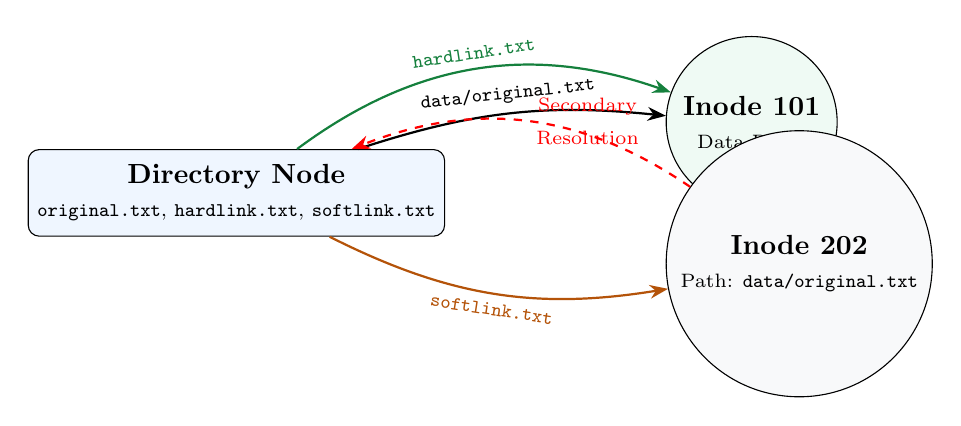
\begin{tikzpicture}[>=Stealth, node distance=2.4cm, auto]
    \node[draw, rectangle, rounded corners, fill=softBlue, minimum width=3.4cm, minimum height=1.1cm, align=center] (DIR) 
      {\textbf{Directory Node}\\ \scriptsize \texttt{original.txt}, \texttt{hardlink.txt}, \texttt{softlink.txt}};

    \node[draw, circle, fill=softGreen, right=2.8cm of DIR, yshift=0.9cm, align=center] (INODE1) 
      {\textbf{Inode 101}\\ \scriptsize Data Block};
    \node[draw, circle, fill=softGray, right=2.8cm of DIR, yshift=-0.9cm, align=center] (INODE2) 
      {\textbf{Inode 202}\\ \scriptsize Path: \texttt{data/original.txt}};

    \draw[->, thick] (DIR) to[bend left=12] node[above, sloped] {\scriptsize \texttt{data/original.txt}} (INODE1);
    \draw[->, thick, deepGreen] (DIR) to[bend left=28] node[above, sloped] {\scriptsize \texttt{hardlink.txt}} (INODE1);
    \draw[->, thick, deepAmber] (DIR) to[bend right=18] node[below, sloped] {\scriptsize \texttt{softlink.txt}} (INODE2);
    \draw[->, thick, dashed, red] (INODE2) to[bend right=28] node[right, align=center] {\scriptsize Secondary\\ \scriptsize Resolution} (DIR);
  \end{tikzpicture}
  \caption{Naming graph illustrating direct inode binding (hard link) vs. path indirection (soft link).}
  \label{fig:naming_graph}
\end{figure}

\begin{solutionbox}[Theoretical Explanation of Results]
\begin{itemize}[leftmargin=*,itemsep=1pt]
  \item \textbf{Hard Links Participate Directly in the Naming Graph:} \texttt{data/original.txt} and \texttt{hardlink.txt} share the identical inode number (\texttt{7881299348562163}) with link count 2. Renaming or deleting the original file merely unlinks that specific directory entry and decrements the inode reference count to 1; the data blocks remain fully accessible via \texttt{hardlink.txt}.
  \item \textbf{Soft Links Introduce Fragile Indirection:} The symbolic link is a separate inode (\texttt{9288674232115449}) whose payload is a text path string. Renaming \texttt{original.txt} to \texttt{renamed.txt} leaves the soft link pointing to a non-existent path string, producing an unresolvable \textbf{dangling reference} (\texttt{ENOENT: No such file or directory}).
\end{itemize}
\end{solutionbox}

% ================================================================
\section{Comparative Synthesis of Naming Schemes}
% ================================================================

\begin{table}[H]
\centering
\caption{Dimensional comparison of distributed naming and location mechanisms}
\label{tab:comparison}
\footnotesize
\begin{tabular}{p{2.6cm}p{2.3cm}p{2.3cm}p{3.2cm}p{4.0cm}}
\toprule
\textbf{Mechanism} & \textbf{Lookup Latency} & \textbf{Update Cost} & \textbf{Scalability} & \textbf{Failure Vulnerability} \\
\midrule
\textbf{Broadcast (ARP/UDP)} & $O(1)$ RTT (LAN) & $O(1)$ (no tables) & Low (bounded by local subnet) & Resilient to crashes; vulnerable to packet storms \\
\addlinespace
\textbf{Forwarding Pointers} & $O(k)$ hops & $O(1)$ at prior node & Low (chains lengthen with mobility) & High (single intermediate failure severs chain) \\
\addlinespace
\textbf{DHT / Chord Ring} & $O(\log N)$ hops & $O(\log^2 N)$ updates & High (scales to millions of nodes) & Robust through finger stabilization and successor lists \\
\addlinespace
\textbf{HLS (Hierarchical)} & $O(\text{height})$ (to LCA) & Localized to LCA & Very High (exploits geographic locality) & High-level failures impede wide-area lookups \\
\addlinespace
\textbf{FS Hard Links} & $O(1)$ direct inode & $O(1)$ refcount & Single file system partition & High durability (data preserved while refcount $>0$) \\
\addlinespace
\textbf{FS Soft Links} & $O(\text{path length})$ & $O(1)$ string write & Cross-device / distributed mounts & Fragile (renaming target yields dangling reference) \\
\bottomrule
\end{tabular}
\end{table}

% ================================================================
\section{Conclusions}
% ================================================================

\begin{enumerate}[leftmargin=*,itemsep=1pt]
  \item \textbf{Identity vs. Location:} Identifiers provide permanent, location-independent entity keys, whereas addresses provide topological routing endpoints. Effective distributed systems must cleanly decouple identity from physical access points.
  \item \textbf{Flat vs. Hierarchical Trade-offs:} While broadcast provides zero-configuration discovery on LANs, it cannot cross network boundaries. Structured approaches like Chord achieve logarithmic $O(\log N)$ scalability through consistent hashing.
  \item \textbf{Locality Exploitation:} Hierarchical architectures like HLS confine queries and update signaling to the lowest common ancestor (LCA), protecting higher-level infrastructure from regional bottlenecks.
  \item \textbf{Graph-Theoretic Naming:} Direct inode references (hard links) provide crash resilience and data retention, whereas indirect path resolution (soft links) offers cross-filesystem flexibility at the expense of dangling pointers.
\end{enumerate}

% ================================================================
\begin{thebibliography}{9}
\small
\bibitem{tanenbaum}
A.~S.~Tanenbaum and M.~van~Steen, \textit{Distributed Systems: Principles and Paradigms}, 3rd ed., 2017.

\bibitem{coulouris}
G.~Coulouris, J.~Dollimore, T.~Kindberg, and G.~Blair, \textit{Distributed Systems: Concepts and Design}, 5th ed., 2011.

\bibitem{chord}
I.~Stoica et al., ``Chord: A scalable peer-to-peer lookup service for internet applications,'' \textit{ACM SIGCOMM}, 2001.

\bibitem{hidrobo}
F.~Hidrobo, ``Workshop 3: Naming --- Distributed Systems,'' Yachay Tech University, Semester II, 2026.
\end{thebibliography}

\end{document}
